\documentclass[12pt,ngerman,parskip=half]{scrartcl}
%Ich bin ein Kommentar
% article, report und book sind US/englische Klassen.
% Im deutschsprachigen Raum sind KOMA Klassen besser


\author{Uwe Ziegenhagen}
\title{Mein erstes LaTeX-Dokument}

\usepackage{babel}
\usepackage{blindtext}
\usepackage{microtype}
\usepackage{graphicx}

\usepackage{hyperref}
\hypersetup{
    bookmarks=true,                     % show bookmarks bar
    unicode=false,                      % non - Latin characters in Acrobat’s bookmarks
    pdftoolbar=true,                        % show Acrobat’s toolbar
    pdfmenubar=true,                        % show Acrobat’s menu
    pdffitwindow=false,                 % window fit to page when opened
    pdfstartview={FitH},                    % fits the width of the page to the window
    pdftitle={My title},                        % title
    pdfauthor={Author},                 % author
    pdfsubject={Subject},                   % subject of the document
    pdfcreator={Creator},                   % creator of the document
    pdfproducer={Producer},             % producer of the document
    pdfkeywords={keyword1, key2, key3},   % list of keywords
    pdfnewwindow=true,                  % links in new window
    colorlinks=true,                        % false: boxed links; true: colored links
    linkcolor=blue,                          % color of internal links
    filecolor=blue,                     % color of file links
    citecolor=blue,                     % color of file links
    urlcolor=blue                        % color of external links
}

\begin{document}
\maketitle

\tableofcontents

\pagebreak % \newpage

\listoffigures

\section{Einleitung}\label{sec:Einleitung}
\subsection{Literatur}

\subsubsection{Deutschland}

Hallo DLR!

Hallo DLR, ich bin ein Satz. Ich bin der zweite Satz im gleichen Absatz.

Hallo DLR, ich bin ein Satz.  Ich bin der zweite Satz im gleichen Absatz.

% PDF kann PDF, JPG und PNG
\begin{figure}
\begin{center}

\includegraphics[width=0.8\textwidth]{Bilder/Katze}
\caption{Melli 1}\label{fig:Katze}
\end{center}
\end{figure}

\blindtext[10]


\begin{figure}
\begin{center}
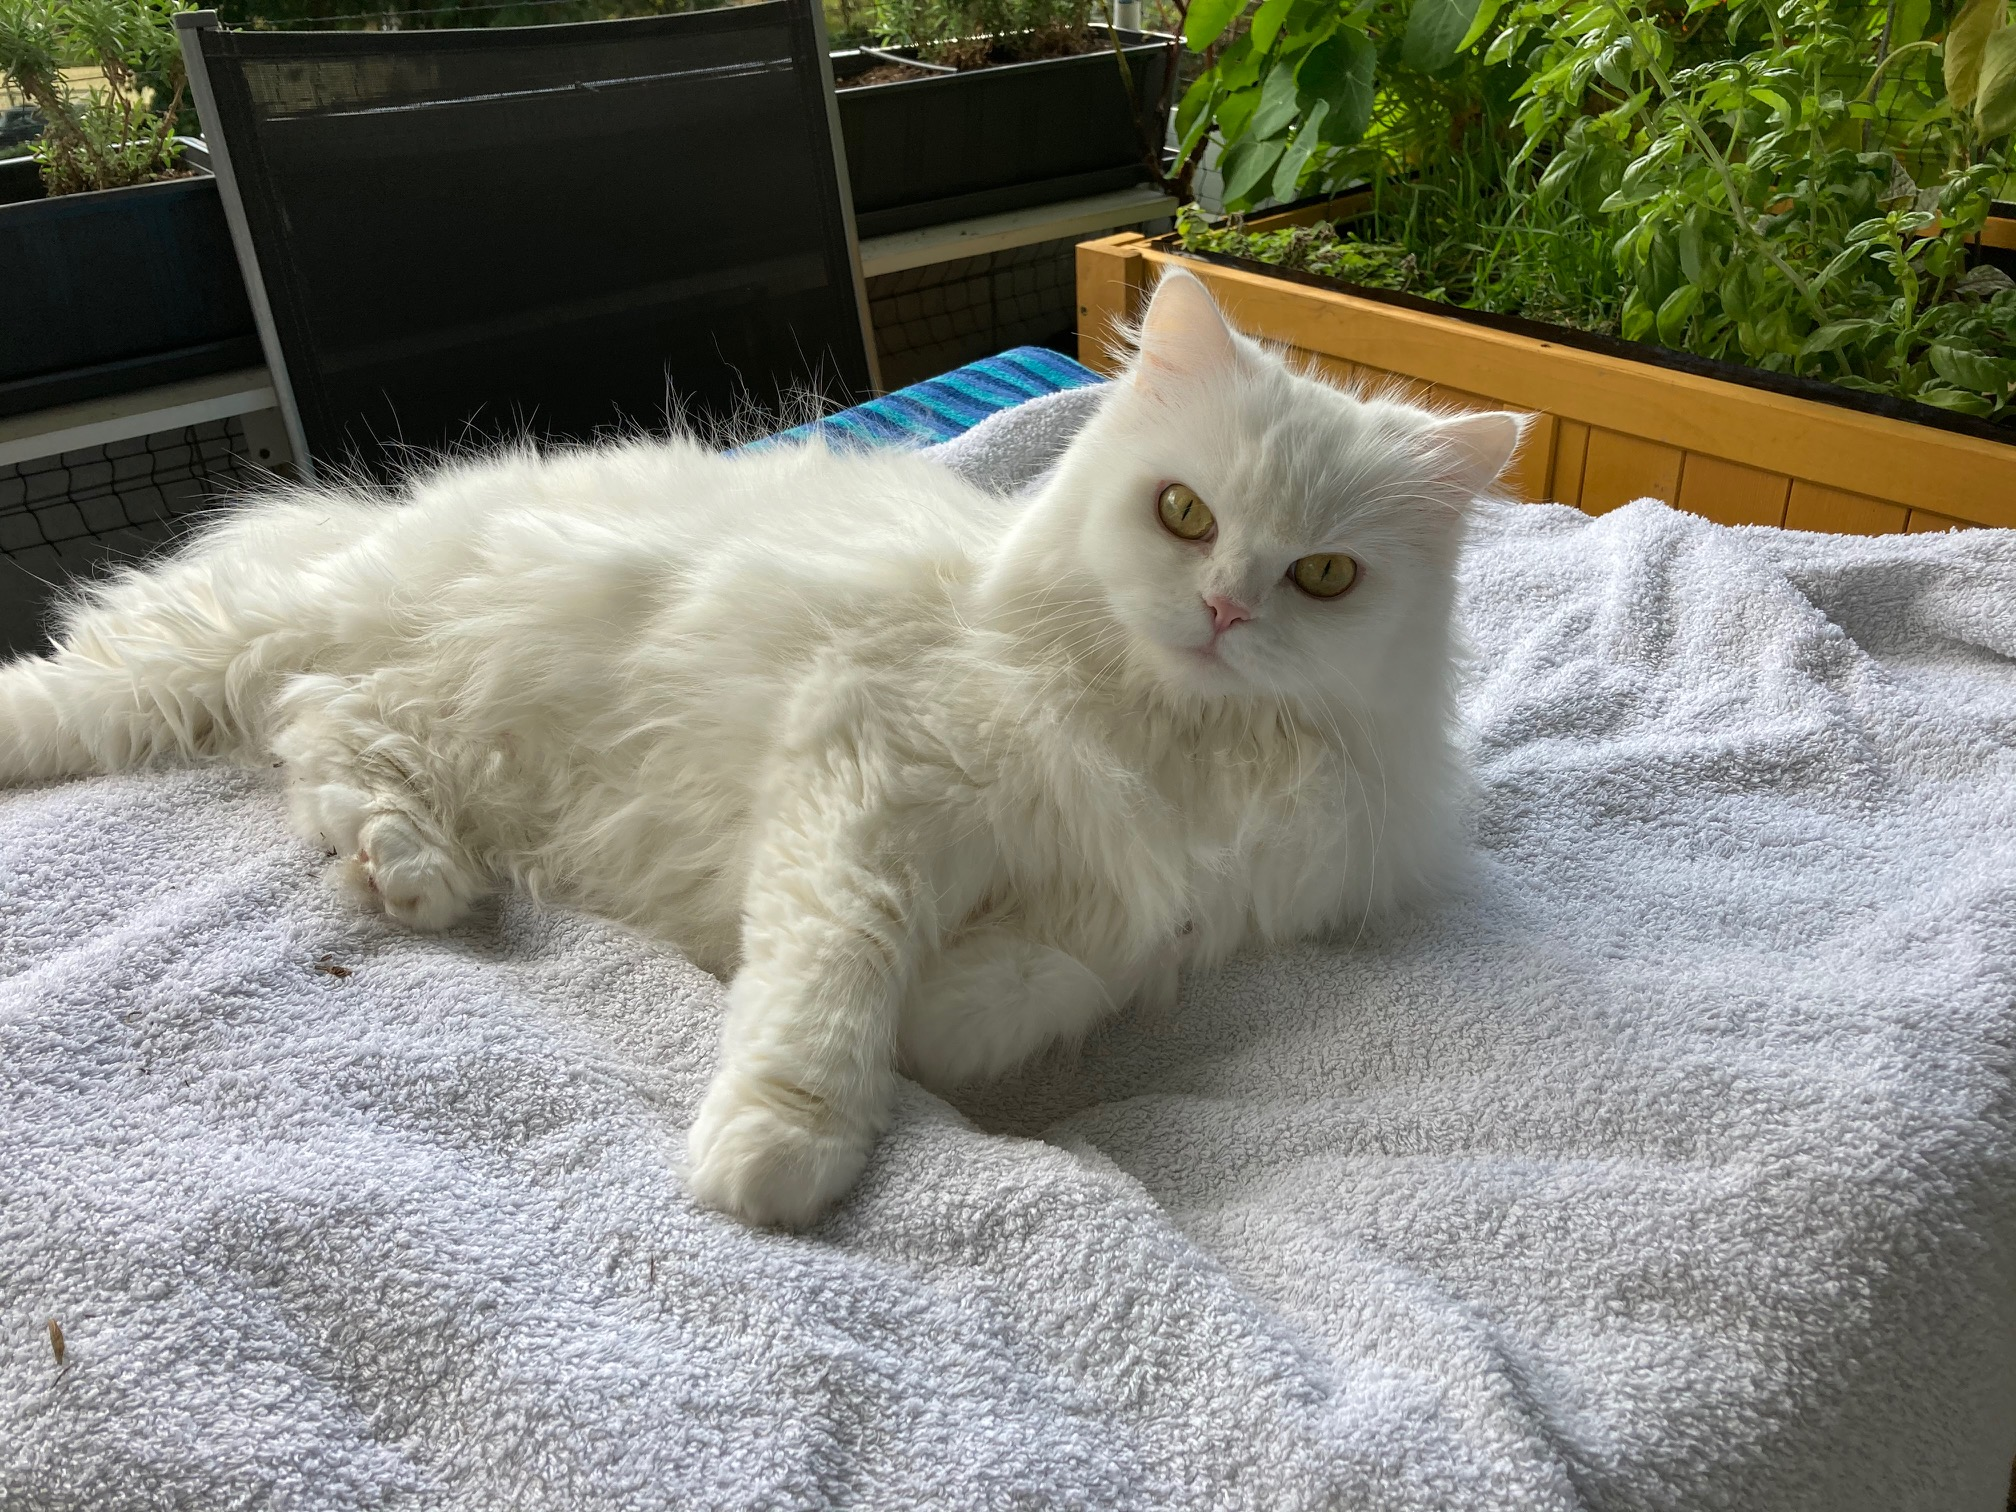
\includegraphics[width=0.8\textwidth]{Bilder/Katze1}
\caption{Melli 2, \blindtext}
\end{center}
\end{figure}

\blindtext[10]


\begin{figure}
\begin{center}

\includegraphics[width=0.8\textwidth]{Bilder/miau}
\caption{Melli 3}
\end{center}
\end{figure}

\subsubsection{International}

sdfsdfsd


\blindtext

\section{Analyse} 

\blindtext

\blindtext[10]

\section{Fazit}

\blindtext[10]

Siehe Abbildung \ref{fig:Katze} auf Seite \pageref{fig:Katze}

Siehe Abschnitt \ref{sec:Einleitung}
\end{document}
